\documentclass[degree=master, tocarialchapter]{thuthesis}
% 选项
%   degree=[bachelor|master|doctor|postdoctor], % 必选,学位类型
%   secret,                % 可选(默认:关闭),是否有密级
%   tocarialchapter,       % 可选(默认:关闭),章目录中使用黑体(这项表示同时打开下面两项)
%   tocarialchapterentry,  % 可选(默认:关闭),单独控制章标题在目录中使用黑体
%   tocarialchapterpage,   % 可选(默认:关闭),单独控制章页码在目录中使用黑体
%   pifootnote,            % 可选(默认:关闭),页脚编号采用 pifont 字体符号,建议打开

% 所有其它可能用到的包都统一放到这里了,可以根据自己的实际添加或者删除。
\usepackage{thuthesis}

% 定义所有的图片文件在 figures 子目录下
\graphicspath{{figures/}}

% 可以在这里修改配置文件中的定义。导言区可以使用中文。
% \def\myname{薛瑞尼}

\begin{document}

%%% 封面部分
\frontmatter
\thusetup{
  %******************************
  % 注意:
  %   1. 配置里面不要出现空行
  %   2. 不需要的配置信息可以删除
  %******************************
  %
  %=====
  % 秘级
  %=====
  secretlevel={秘密},
  secretyear={10},
  %
  %=========
  % 中文信息
  %=========
  ctitle={基于多步决策的文本情感识别},
  cdegree={工学硕士},
  cdepartment={计算机科学与技术系},
  cmajor={计算机科学与技术},
  cauthor={梁锡豪},
  csupervisor={徐明星副教授},
  % cassosupervisor={陈文光教授}, % 副指导老师
  % ccosupervisor={某某某教授}, % 联合指导老师
  % 日期自动使用当前时间,若需指定按如下方式修改:
  % cdate={超新星纪元},
  %
  % 博士后专有部分
  % cfirstdiscipline={计算机科学与技术},
  % cseconddiscipline={系统结构},
  % postdoctordate={2009年7月——2011年7月},
  % id={编号}, % 可以留空: id={},
  % udc={UDC}, % 可以留空
  % catalognumber={分类号}, % 可以留空
  %
  %=========
  % 英文信息
  %=========
  etitle={Multi-step-decision-making Based Text Sentiment Analysis},
  % 这块比较复杂,需要分情况讨论:
  % 1. 学术型硕士
  %    edegree:必须为Master of Arts或Master of Science(注意大小写)
  %             “哲学、文学、历史学、法学、教育学、艺术学门类,公共管理学科
  %              填写Master of Arts,其它填写Master of Science”
  %    emajor:“获得一级学科授权的学科填写一级学科名称,其它填写二级学科名称”
  % 2. 专业型硕士
  %    edegree:“填写专业学位英文名称全称”
  %    emajor:“工程硕士填写工程领域,其它专业学位不填写此项”
  % 3. 学术型博士
  %    edegree:Doctor of Philosophy(注意大小写)
  %    emajor:“获得一级学科授权的学科填写一级学科名称,其它填写二级学科名称”
  % 4. 专业型博士
  %    edegree:“填写专业学位英文名称全称”
  %    emajor:不填写此项
  edegree={Doctor of Engineering},
  emajor={Computer Science and Technology},
  eauthor={Liang Xihao},
  esupervisor={Professor Xu Mingxing},
  % eassosupervisor={Chen Wenguang},
  % 日期自动生成,若需指定按如下方式修改:
  % edate={December, 2005}
  %
  % 关键词用“英文逗号”分割
  ckeywords={情感分析, 反讽识别, 深度学习,集成学习},
  ekeywords={Sentiment analysis, irony detection, deep learning, ensemble learning}
}

% 定义中英文摘要和关键字
\begin{cabstract}

自Web2.0普及后,人们逐渐习惯在互联网的各种平台上分享他们的想法和情感。透过对这些媒体进行情感分析,我们可以得知人们对特定人事物的想法和态度。对人们的想法快速作出响应能够带来相应的商业价值和政治价值,其相关技术也因此得到了重视。而文本作为社交平台上的主要媒体之一,面向文本的情感识别在近年也成为了热门的研究领域。本论文探讨了文本情感识别中的两个问题,主要内容如下:

\begin{enumerate}

\item {\bf 基于多步决策的多分类系统框架}。随着现实中应用场景变得复杂,需要解决的多分类问题越来越多。当区分的类别越多,机器学习算法对数据进行拟合的难度更高,另外对识别性能的要求也变得复杂,譬如确保个别类别的召回率和正确率等。为此,我们提出了一种基于多步决策的多分类系统框架,把一个多分类问题拆解成多个子分类问题的叠加,再透过逐步回答每个子问题得出最终的识别结果。由于识别过程中每一步只关注一个子分类问题,我们能从局部调整系统的识别能力,并针对特定的评价指标进行优化。另一方面,每个子分类问题可以分别采用不同的算法,以此结合不同模型能捕捉到的不同信息。

\item {\bf 用于结合上下文的多通道模型}。在某些场景下,仅凭一段文本无法准确了解发言者想表达的意思和态度。为了处理这种情況,一些文本情感识別研究会引入上下文作为提示。为此我们提出了一种多通道模型框架,让对识别目标起不同作用的上下文先分别经过不同的编码器进行编码提取出有用的特征,再考虑合并正文和上下文的信息得出识别结果。

\end{enumerate}

为了验证基于多步决策的多分类系统框架,我们首先将其应用于面向微博的反讽识别,根据国际比赛SemEval-2018的任务三进行实验,结果显示我们的模型超过了当时排名第一的系统。
另外为了验证我们提出的多通道分类模型,我们将其应用于面向三轮对话的情感识别,根据公开比赛SemEval-2019的任务三进行实验,结果显示我们的模型达到了当时排名前十的性能。

% 关键词是为了文献标引工作、用以表示全文主要内容信息的单词或术语。关键词不超过 5
% 个,每个关键词中间用分号分隔。(模板作者注:关键词分隔符不用考虑,模板会自动处
% 理。英文关键词同理。)

\end{cabstract}

% 如果习惯关键字跟在摘要文字后面,可以用直接命令来设置,如下:
% \ckeywords{\TeX, \LaTeX, CJK, 模板, 论文}

\begin{eabstract}

Since the poularization of Web 2.0, people get used to share they thoughts and emotions on different online platforms. By analyzing the sentiment of these data, we can have an in sight into the people's opinion towards certain things. Vast commercial and political values can be obtained through quick response to the people's attitude. Therefore related technologies are getting more attention. As text is one of the mostly used media on social platforms, text sentiment analysis has become a popular research field. This thesis explores two problems in text sentiment analysis and it is organized as follows:

\begin{enumerate}

\item {\bf Multi-step-decision-making based multi-classification system framework}. As real-world application scenes are becoming more complex, more multi-classification problems are encountered. As the data are divided into more categories, it becomes more difficult for machine learning algorithms to fit the data. On the other hand, the requirement of predictive performance are getting more complicated, such as ensuring the recall rate and the precision level of certain categories. Hence, we propose a multi-step-decision-making based multi-classification system framework, which disassembles a multi-classification problem into a sequence of sub-classification problems and classifies an object by answering the sub-questions step by step. As the classification system only focuses on a sub-problem at each step, its performance can be adjusted locally and we can optimize the overall performance for certain evaluation metrics. On the other hand, algorithms can be chosen for each sub-problem individually, hence the information captured by different kinds of models can be combined in the system.

\item {\bf Multi-channel model for manipulating contextual information}. Sometimes we may not exactly understand what a person want to express or how he feels only through his written message. To deal with this problem, some of the text sentiment analysis researches take into account the contextual clues. Therefore, we propose a multi-channel model. By feeding contextual information that play different parts of role into different feature encoders, features of different parts of the context are encoded and further combined with that of the main message to get the identification result.

\end{enumerate}

To verify the effectiveness of the proposed multi-step-decision-making based multi-classification system framework, we first apply it to irony detection in English tweets. Experiments are launched based on SemEval-2018 Task 3. Results show that our system exceeds the performance of the no. 1 participating system. On the other hand, to verify the effectiveness of our multi-channel model, we apply it to contextual emotion detection in text. Experiments are launched based on SemEval-2019 Task 3. Results show that our system reaches the top 10 performance among the participants.

\end{eabstract}

% \ekeywords{\TeX, \LaTeX, CJK, template, thesis}

% 如果使用授权说明扫描页,将可选参数中指定为扫描得到的 PDF 文件名,例如:
% \makecover[scan-auth.pdf]
\makecover

%% 目录
\tableofcontents

%% 符号对照表
\begin{denotation}[3cm]

\item[BOW] 词袋模型 (Bag of Words)
\item[BP] 反向传播算法 (Back-propagation)
\item[BRNN] 双向递归神经网络 (Bidirectional Recurrent Neural Network)
\item[CRF] 条件随机场 (Conditional Random Field)
\item[GRU] 门控循环神经元 (Gated Recurrent Unit)
\item[LSTM] 长短时记忆网络 (Long Short-Term Memory)
\item[POS] 词性 (Part-of-speech)
\item[RNN] 递归神经网络 (Recurrent Neural Network)
\item[SVD] 奇异值分解 (Singular Value Decomposition)
\item[SVM] 高性能计算 (High Performance Computing)
\item[TF-IDF] 词频-逆文档频度 (Term Frequency - Inverse Document Frequency)
\item[ReLU] 线性整流函数 (Rectified Linear Unit)

\end{denotation}




%%% 正文部分
\mainmatter
\chapter{引言}
\label{cha:intro}

\section{研究背景与意义}

情感识别旨在了解人们对特定事件或实体的态度和情感。自Web2.0普及后,大量网民每天在互联网生产着各种各样的内容,其中包含不同方面的信息,如个人生活经历,购买行为,对产品服务的体验评价,对社会时事的看法等等。从人们的日常社交需求来看,这种借由互联网媒体的分享非常便捷,我们可以了解到亲朋好友的近况,也可以和不认识的网民交流对具体事件的想法。在商业上,借由对用户的网络行为进行分析,企业可以对他们的客户或者潜在客户有更深入的了解,对他们的需求和反馈及时作出反应将带来战略性的优势。在社会管理上,政府可以透过对网民在网络上的发言了解人民的想法和舆论的走向,进而作出相应的措施。正因为互联网的普及,才使得以上基于对特定人群的了解来进行决策的做法成为可能。随着数据资源变得丰富,相应的技术在近年得以快速发展,目前市面上已经有公司(如国内的腾讯和阿里巴巴,以及国外的微软和亚马逊等)提供基于大型社交媒体平台(如微博、讨论区等)上的数据进行情感分析相关的规泛化服务,然而相应的技术依然有进步空间,研究工作还在不同方向上摸索。

情感在人们的思想表达和交流中起着重要作用\cite{Banerjee2015Detection},比起了解该想法的细节内容,情感对应该想法的一种倾向。譬如在分析用户对新产品的评论时,
只需要分析其中褒贬意思的倾向即可大致了解新产品是否能让大部分的客户满意,或者筛选出其中表示不满意的用户再进行深入分析,因此情感识别技术具有一定的应用价值。而由于在互联网上,大部分情况下用户以文本表达想法,面向文本的情感识别成为了近年最重要的研究课题之一。相对于人们面对面交流的场景,聆听者可以根据发言者的肢体语言、面部表情以及声调变化等额外信息更好地理解发言者想表达的意思,然而这些信息并不存在于文本当中,这也正是对文本进行情感识别本身的难点之一\cite{SemEval2019Task3}。

情感识别的另一个难点在于语言中丰富多样的修辞手法,其中反讽是具代表性的修辞手法之一。Henry Watson Fowler在《The King's English》一书中描述“即使对反讽的定义有数百种, 其中只有包含'表面意思和实际意思不同'这个概念的才能被接受”。Eric Partridge 在《Usage and Abusage》一书中指出“反讽存在于所表达意思的另一面”。总的多说当反讽在文本中出现,那么发言者想表达的意思应该和文本的字面意思完全相反。譬如某人表示“我就喜欢你不断挑战我的底线”,在字面上“喜欢”表达的是正面的情感,然而根据常识可知“挑战底线”是一种让人反感的行为,与“喜欢”相矛盾。这段文字实则表示发言者正被某人触及底线,表达的是负面情感。所以在情感识别当中,正确识别出反讽的使用能够避免对内容的错误理解,反讽识别因此成为了和情感识别紧密相关的研究课题。

\section{国内外研究现状}

\subsection{情感模型}

情感计算的基础是对情感作出描述,现有的描述方式可以分成两个大类: 范畴观和维度观。范畴观即把不同情感对应到一组离散的情感标签上,其中具代表性的有Plutchik的情感模型\cite{Plutchik1980Emo}和Ekan的情感理论\cite{Ekman1992An}。Plutchik的情感模型包含八种情感:愤怒、恐惧、悲伤、厌恶、期待、信任、高兴、惊讶;这些情感都各自对应具有重要生存意义的行为,各种复杂的情感都是由这此基本情感构成,另外这八种情感可以分成四组对立的情感对。Ekan在十年后提出的情感理论和Plutchik的相似,但相对地少了期待和信任两种情感,是一个六类情感模型。

\begin{figure}[h]
  \centering%
  \subcaptionbox{三维模型\label{fig:plutchik_emotion_wheel_3d}} %[3cm] 标题的长度,超过则会换行,如下一个小图。
    {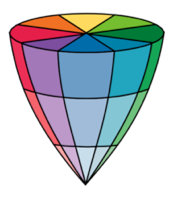
\includegraphics[height=4cm]{img/plutchik_3d.png}}%
  \hspace{4em}%
  \subcaptionbox{二维模型\label{fig:plutchik_emotion_wheel_2d}}
      {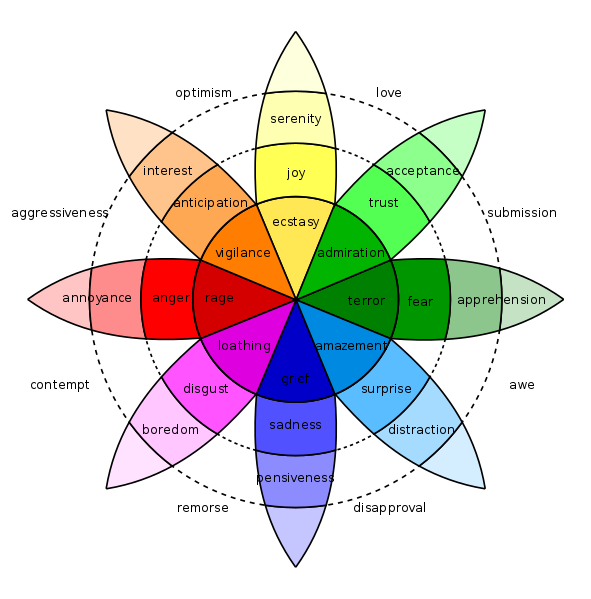
\includegraphics[height=8cm]{img/plutchik_2d.png}}
  \caption{Plutchik\cite{Plutchik1980Emo}提出的情感轮模型}
  \label{fig:plutchik_emotion_wheel}
\end{figure}

以维度观描述情感就是把情感映射到多维空间的点上,而目前维度观情感模型以二维和三维空间的为主。二维情感模型中较有代表性的是Russell提出的环状模型(Circumplex Model)\cite{Russell1980Cir} ,其中纵坐标对应情感的激活度(Arousal),横坐标对应情感向性(Valence),而不同的情感则分布在一个环状的区域内。Bradley等人\cite{Bradley1992Rem}提出的向量模型(Vector Model)在对横轴和纵轴的定义和前者相似,但其理论假设高激活度的情感应该有较明显的正负倾向,相对地低激活度的情感则偏向中性,故情感分布在一个回力标形状的区域。Watson和Tellegen \cite{Watson1985Tow} 提出的 PANA(positive activiation-negative activation)模型和前两者在理论基础上则有明显的不同,他们认为情感的正面作面和负面作用是两个独立的成分,所以在模型中纵轴和横轴分别表示情感正面作用和负面作用的强弱,不过该模型相当于把Russell等人提出的环状模型的向量空间旋转45度\cite{Rubin2009A}。

基于三维空间的情感模型中具有代表性的有Plutchik\cite{Plutchik1980Emo}提出的情感轮模型,Plutchik认为情绪之间包含强度,相似性和两极性三种维度,椎体的顶部和底部分别对应强的情感和弱的情感,相似的情感对应椎体中相近的位置,对立的的情绪则会对应到椎体中对立的位置上。另外还有Mehrabian \cite{Mehrabian1996Pleasure}提出的PAD模型,其三维空间的三个坐标轴分别对应情感愉悦度(Pleasure)、激活度(Arousal)以及优势度(Dominance)。较近期被提出的是Hugo\cite{Hugo2012A}的情感立方体模型,其三维空间的三个坐标轴分别对应5-羟色胺(5-hydroxytryptamine, 5-HT), 多巴胺(dopamine,DA)和去甲肾上腺素(noradrenaline,NE)三种神经递质所产生信号的强弱,并对空间中一个立方体的八个顶点标记了其对应的情感。

\begin{figure}[H] % use float package if you want it here
  \centering
  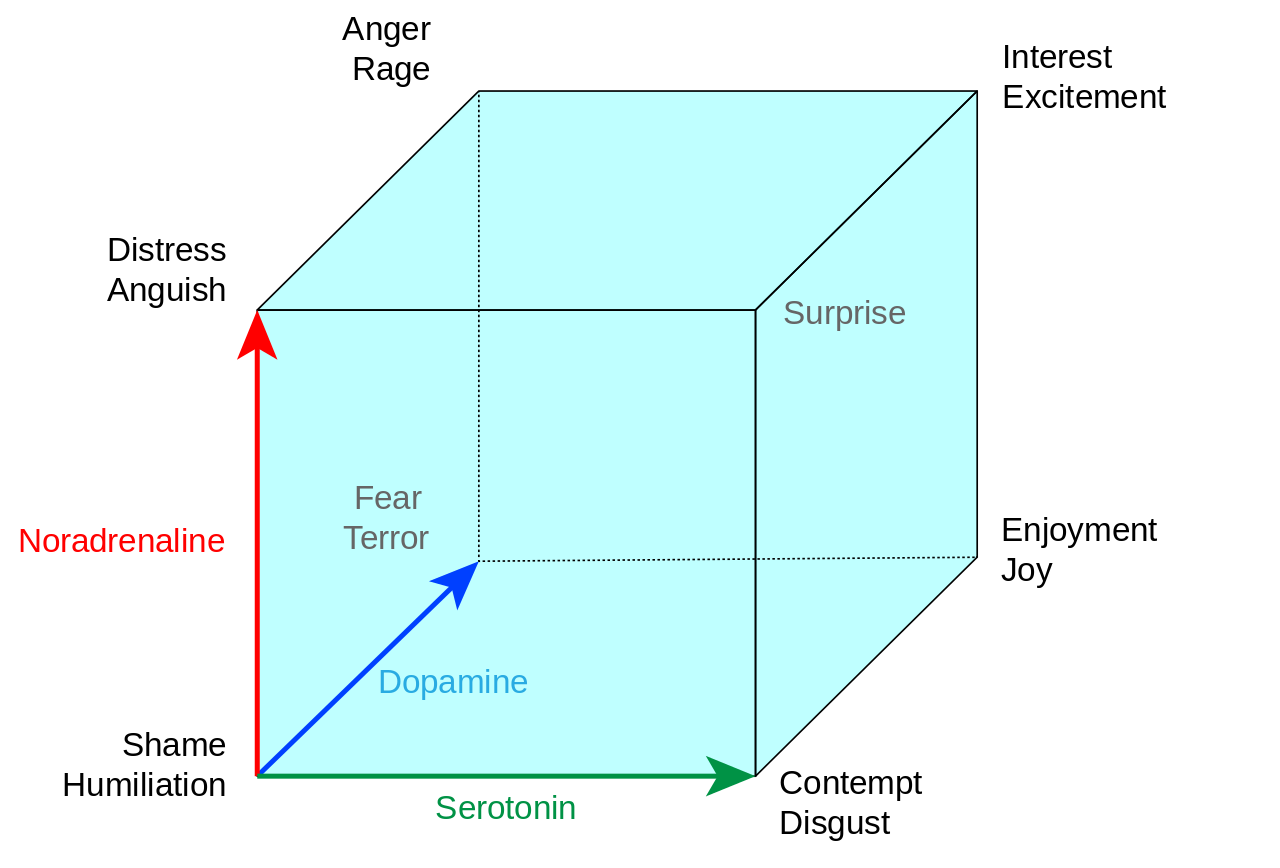
\includegraphics[width=0.8\textwidth]{img/hugo_cube_of_emotion.png}
  \caption{Hugo\cite{Hugo2012A}提出的情感立方体模型}
  \label{fig:hugo_cube_of_emotion}
\end{figure}

\subsection{情感识别}

对应上述情感模型的分类,情感识别研究可以分成两类。第一类对应范畴观,给定一组情感类型,判断一段文本中所表达的情感倾向于该组情感中的哪一种,或者是否包含这一组情感中的一种或多种情感。如国际比赛SemEval-2018任务一\cite{mohammad2018semeval}的子任务要求识别一段微博中是否包含愤怒、恐惧、悲伤等十一种情感中的一种或多种情感。另一类情感识别研究对应维度观,对于给定的情感属性,判断一段文本中该情感属性的强度。其中常见的有情感向性的二分类问题(正性或负性)、三分类问题(正性、中性或负性)、五分类问题(非常正性,正性、中性、负性或非常负性)。其中五分类问题的研究对象一般是互联网上五星评分制的产品评论或者电影评论等。

另一方面,目前文本情感识别的研究按照文本的粒度可以大致分成三类:文章级别、句子级别、属性级别。在文章级别的情感识别中,虽然一篇文章由多个句子组成,但假设整篇文章存在某种情感倾向,而研究目标则是自动识别出该种情感倾向的类型或强度。Turney \cite{turney2002thumbs} 利用线上电影评论中"推荐"(大拇指朝上)和"不推荐"(大拇指朝下)的标记研究对电影评论的正负性情感识别。他提出利用点互信息(Pointwise Mutual Information,PMI)来评估单词的语义倾向性,其中PMI透过在大型语料库中统计两个单词共同出现的情况来评估两个单词的相似度。首先利用PMI值评估各个单词与正向情感的代表性单词"excellent"和负向情感的代表性单词"poor"的相似性,再取这两个PMI值作差得出该单词在语义上倾向于哪一种情感,再透过计算整段评论的平均语义倾向性评估整体的情感倾向。Pang和Lee \cite{pang2004sentimental} 采用了不同的方法研究相同的问题。他们首先对评论中每个句子的主观程度进行评分,利用评分构造一个带权重的句子关系图,再基于最小割算法结合上下文加强对每个句子主观程度的判断,过滤评论中不带主观情感的句子后再判断整个评论的情感向性,以此加强识别效果。Tang等人 \cite{tang2015learning} 则研究了产品评论的五级评分预测。除了评论的文本内容,他们进一步引入了用户的信息和产品的信息。经过数据分析,他们发现相同用户对不同产品的评论和评分比不同用户之间的更一致,另外不同用户对同一产品的评论和评分比不同产品之间的更一致,这显示了用户和产品各自都存在一些相对固定的属性。因此Tang等人提出一种为用户和产品生成表示向量的方法,并应用于评论的五级评分预测。实验结果显示他们的方法在多个数据集上达到了较好的性能,这同时引出了加入背景信息来加强系统识别能力的可能性。

然而一篇文章有可能同时表达了多种观点和情感,因此有另一类研究针对句子或短文本所表达的情感,即句子级别的情感识别。由于句子的文本长度较文章的短,文本内部的逻辑较简单,但相对地所包含的提示信息也较少,课题的难点与前者有所不同。Khan等人\cite{khan2011sentiment}研究了对线上评论中句子进行正负性情感识别。他们首先区分出评论中各个句子的主观性和客观性,然后针对带主观情感的句子,利用开源自然语言工具SentiWordNet获取各个单词的正负情感属性,再根据句子的词性标注和他们设计的规则计算整个句子的情感向性。Khan等人默认单词的正负情感属性在不同场景下不变,然而Li等人\cite{li2013constructing}指出部分单词在特定场景下会有不同的情感向性,因此他们提出了一种有监督学习方法,自动学习各单词在指定领域下的情感向性,以此作为文本的特征,并应用于对产品评论的情感识别中。实验结果显示使用SentiWordNet提供的全局情感评分和针对领域评估的情感评分相比,使用后者能达到的识别性能力更好,验证了他们的假设。一些研究则选择端到端地学习单词的情感和语义倾向,在Santos和Gatti\cite{dos2014deep}对电影评论和微博的情感识别研究中,他们提出了利用卷积神经网络分别从字符级别和词级别计算出单词对应的特征向量,然后同样以卷积神经网络结合句子中各单词的向量得出句子的表示向量和预测整体的情感倾向。结果显示他们的方法较早期的其他方法性能更好。

在一些应用场景当中,我们希望了解发言者对某个对象或者它的某个特定属性的想法。譬如新手机推出市场后,厂商需要了解用户对手机的续航能力、拍照质量、交互体验等各方面的评价,那么对于评论中同时谈论手机的多个属性且好评和差评不一时,应该针对各个属性分别识别发言者所表达的感情,因此有了属性级别的情感识别。Che等人\cite{che2015sentence}提出一种句子压缩算法,透过对句子进行依存句法分析,过滤与目标属性的情感无关的内容。他们采用了多种语义和语法特征作为输入,以条件随机场(Conditional random field,CRF)作为分类器。实验结果显示过滤掉不相关的文本部分后,识别性能有所提升。Wang等人\cite{wang2016attention}研究了对网上评论中特定实体或属性的情感识别。他们提出了一个基于注意力机制的长短时记忆网络(Long Short-Term Memory,LSTM),特点在于只以词向量作为输入,而不采用其他传统的语义和语法特征,另外利用注意力机制自动识别与目标相关的内容。他们的实验基于国际比赛SemEval-2014任务四\cite{pontiki2014semeval}中的一个子任务,结果然显示他们的系统性能达到了当时的技术水平。另外透过对注意力单元的输出进行分析,验证了注意力机制能够有效识别文本中与目标相关的内容。Tang等人\cite{tang2016aspect}分别对前述数据集中电脑和餐庁相关的两组样本进行属性级别的情感识别,但有别于当时主流的以特征提取为主的浅层机器学习方法(如支持向量机)和针对序列的深度学习模型(如递归神经网络),他们提出了一个基于注意力机制的深度记忆网络。另外针对文本中各个单词和目标单词在句子中的距离,作者引入了距离信息提出了注意力单元的多种变形。实验结果显示他们提出的深度记忆网络达到了当时第一名参赛系统(基于手工特征和支持向量机的算法)的性能。另外对注意力单元的中间结果进行人工分析,验证了在同一段评论中,引入距离信息的注意力单元有助于区分不同单词对不同目标的情感的贡献。

\subsection{反讽识别}

正如前面所述,反讽识别和情感识别紧密相关,识别出反讽的使用对正确识别情感起着关键作用。Tsur等人\cite{tsur2010icwsm}\cite{davidov2010semi}研究了对微博平台Twitter上的微博以及电商平台亚马逊上的评论进行反讽强度的识别,从明显不含反讽到明显表示反讽分成五级,由人工进行标注。他们提出的SASI算法分别从文本提取了词频相关的模式特征以及基于标点符号的特征,以K最近邻算法作为分类器。另外利用在Twitter按井号标签\#sarcastic自动爬取了额外的反讽语料用于初步的模型训练。对实验结果的比较证明了各种特征的有效性以及添加额外语料对模型训练的帮助。

为了以较低成本获取大量的反讽相关语料,很多研究从微博平台根据井号标签自动筛选出可能带反讽的微博。Reyes等人 \cite{reyes2013multidimensional} 利用\#irony,\#education, \#humor, \#politics在Twitter上自动获取四组不同主题的微博,并把\#irony对应的微博和另外三组微博两两组合进行二分类实验。他们提出了四个方面的文本特征提取方法,包括:特殊标记(词汇和标点符号等)、不可预期性、表达风格、情感特性;并比较了每项特征在各组微博中的出现情况,显示了各项特征和反讽的相关性。另外分别采用朴素贝叶斯和决策树作为分类器,但没有明显的性能区别。

类似的数据收集方法对其他语言同样适用。Kunneman等人\cite{kunneman2015signaling}则利用对应的德语井号标签来获取反讽语料,以此研究德语微博中的反讽识别。他们取N元语法作为输入特征,以Balanced Winnow \cite{littlestone1988learning}作为分类器,在测试集上达到约0.85的召回率和0.87的AUC值。但他们进一步经过人工检验评估了基于井号标签自动标注的有效性,分析结果显示该方法获取的反讽样本中包含约10\%的躁声。

有别于早期以手动设计的特征作为输入和以传统机器学习方法建模,Poria等人 \cite{poria2016deeper} 首次将神经网络应用于对微博的反讽识别。他们的算法框架主要包含四个卷积神经网络,并分别利用不同的数据集进行预训练,分别对应反讽识别、情感极性识别、情感类型识别和性格识别。最后取四个卷积神经网络的中间结果作为特征,利用支持向量机(Support Vector Machine, SVM)进行后融后得出最终预测结果。实验显示引入反讽识别以外的三个语料库提升了系统的识别能力。

\begin{figure}[H] % use float package if you want it here
  \centering
  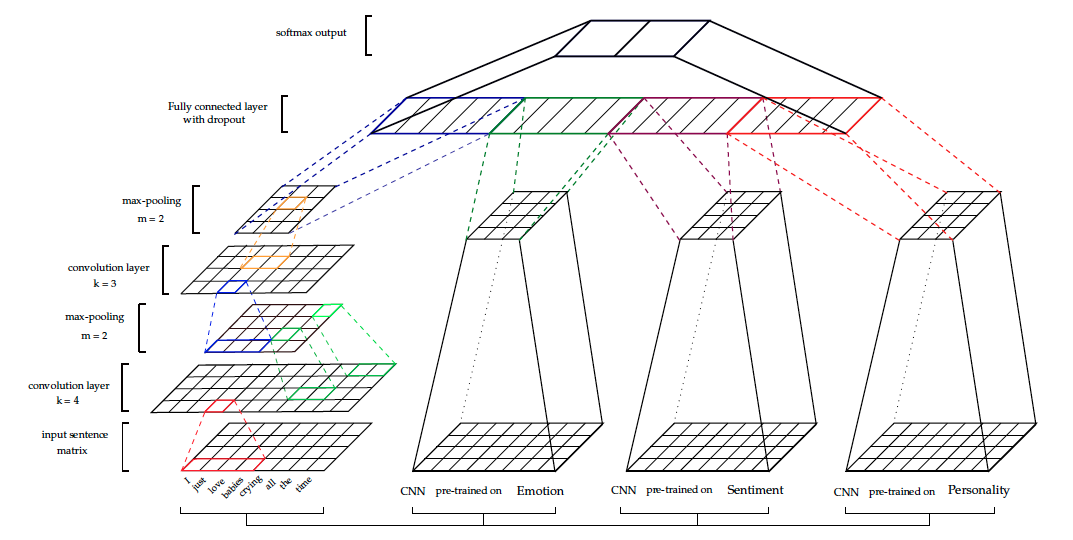
\includegraphics[width=\textwidth]{img/poria2016deeper.png}
  \caption{引入多个领域信息的反讽识别神经网络模型,引自\cite{poria2016deeper}}
  \label{fig:poria2016deeper}
\end{figure}

\subsection{社交媒体上的文本情感识别}

随着社交媒体的普及,网民们习惯于在微博、讨论区等平台上表达个人意见和互相讨论。有别于新闻或学术材料等较正式的文件,网民可以较随心所欲地发言,社交媒体因此成为了情感识别的重要研究对象之一。但和产品评论或文章等文本类型不同,社交媒体上的文本普遍较短\cite{Madhusudhanan2018survey},缺少对背景信息的提示,难以判断其内容所属的主题,这对正确理解其中表达的意思带来困难。另外语言中夹杂着不正规的用法,在中文微博中会出现新的短语或对旧短语有新的解释\cite{xie2012jiyu},如“锦鲤”暗示“好运”,“灌水”表示发表没有意义的内容,在英文微博则中会出现错拼字、非正式缩略语、表情符\cite{go2009twitter}\cite{paltoglou2012twitter},如“tnx”对应英文单词“thanks”,“:)”表示微笑等。虽然没有正式的语言组织对这些新的用法进行整合,但因为这些新用法更方便或对思想的表达更丰富到位,随着在网络上的传播而在网民之间达成了共识。传统的文本特征提取建立在标准的单词使用和正规的语法结构上,而由于新词汇和新语用的出现,导致词汇的意思无法被识别或被错误理解,这对于由人工智能理解文本内容成为了一大难点。因此有别于传统的文本研究,在面向社交媒体的文本情感识别时,需要采用额外手段对文本进行预处理,或透过大量语料尝试自动学习这些新出现的语言属性。

Khan等人\cite{khan2014tom}研究了微博的正负中性情感识别。他们提出了一个混合三个分类器的情感识别框架来解决数据稀疏的问题,另外还提出了一组针对微博文本的预处理步骤,其中包括俚语和缩略语分析、词干提取、拼写检查和修正、用户名和井号标签移除等。他们的系统在6个微博数据集上达到了平均83.3\%的F1值以及平均85.7\%的准确率,和同类型技术比较后验证了他们系统以及预处理手段的有效性。

Angiani等人\cite{angiani2016comparison}针对英语微博比较了各种常用的文本预处理技术对情感分析的影响,其中包括单词的规范化、表情符到情感标签的映射、俚语映射、词干提取、停词过滤等。分析显示除了俚语映射以外,其他技术均对情感识别都有正面影响,其中部分技术有助于统一拼写相似的单词,以此关联相同概念的词组。但同时采用所以预处理技术并不保证达到最好的效果,作者指出依然需要根据应用场景和文本的特性做选择。

\begin{figure}[H] % use float package if you want it here
  \centering
  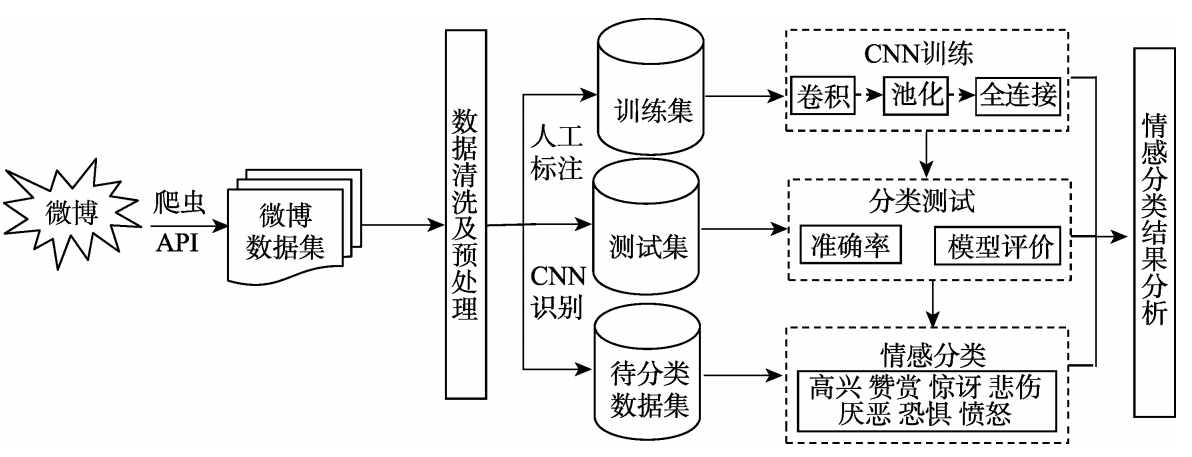
\includegraphics[width=0.8\textwidth]{img/zhang2018jiyu.png}
  \caption{基于卷积神经网络的微博情感分类模型,引自\cite{zhang2018jiyu}}
  \label{fig:zhang2018jiyu}
\end{figure}

张海涛等人\cite{zhang2018jiyu}则研究了中文微博和评论中的文本情感分类。他们针对当时微博上具一定争议性的话题\#打呼噜被室友群殴\#收集数据,确保了样本围绕同一个主题并且有充足的数据量。使用开源工具 NLPIR/ICTCLAS2016 对语料进行分词,再以词向量学习算法word2vec从语料中学习词的表示向量作为输入,以基于卷积神经网络的模型作为分类器,另外以支持向量机作为对照算法。实验结果显示在面向长文本的情感识别时,他们的系统比支持向量机性能更好,而面向短文本时则相反。

\section{存在的问题}

由于近年来各企业或机构对情感识别的需求增加,相关技术的研究备受关注,加上深度学习的快速发展,情感识别和反讽识别的性能水平也在逐年提升。然而相关研究依然存在一些问题需要深入探讨:

\begin{itemize}

\item {\bf 数据不均匀在多分类问题中的影响}。情感识别在早期以识别文本的正性、负性和中性情感为主,但随着应用场景越来越复杂,相关研究逐渐关注其中的细分类别,反讽识别等研究也如此。而在多分类问题中,各类别样本量分布不均匀一直是个备受关注的问题。因为在真实应用场景的多分类问题中,各个类别的样本量往往分布不均匀甚至差别很大,这会导致部分性能指标明显偏低。譬如在训练数据中样本量较少的类别在测试集上的召回率会明显比其他类别的低,间接拉低宏平均的召回率和F1值。然而目前主流的研究工作大部分只探索单个模型如何对多类别的数据进行建模,在人工神经网络领域则是不断提出新的网络结构以在整体上达得到更好的识别能力。另外也有透过数据增强的方法调整训练数据中样本的分布情况,但也难以针对个别类别的识别能力进行调整。

\item {\bf 在算法建模中引入上下文信息} 在一些场景下,仅凭一段文本的内容可能无法完全理解发言者想表达的内容,这在短文本的场景中尤其明显,如微博、评论等。为此目前一些研究会考虑引入文本的上下文,认为这些上下文中包含相关的信息,有助于理解原文的内容。但在不同场景下,上下文的类型不同,其对应建模方式也会有所不同。如在微博平台中,要对微博正文进行情感识别,那么可以引入微博底下的评论以定位该微博描述的事情,另一方面也可以引入用户过去发布的微博,对比他使用表情符的习惯和当前微博中使用的表情符来猜测用户想表达的情感。然而对于不同场景下不同类型的上下文,如何在算法建模中引入上下文信息始终没有一种通用的方法,对于具体的问题依然需要进行针对性的设计。

\end{itemize}

\section{本论文的内容安排}

本文针对上述的两个问题,提出了一个基于多步决策的多分类系统框架以及用于结合上下文的多通道分类模型,并分别基于两个应用场景进行实验以验证他们的有效性。本论文的内容安排如下。

在第\ref{cha:problem_framework}章,我们会对面向文本的情感识别问题作出分析,给出一个统一的数学定义。然后我们会给出一个文本情感识别的研究框架,详细说明其中每一步完成的任务和目的。紧接着会介绍一些自然语言处理和情感识别的相关技术,对于后续实验用中使用到的技术,我们会给出相对充分的说明,另外也会给出相关技术的概要描述,以便于其他研究者在本论文未深入探索的方向进行拓展性的工作。

第\ref{cha:exp_irony_det}章中,我们针对面向微博的反讽识别提出了一种多分类器分层识别算法,同时引出一种针对多分类问题的算法设计框架。我们将基于国际比赛SemEval-2018的任务三\cite{van2018semeval}展开实验,其中包含两个子任务。子任务一为二分类问题,要求识别微博是否包含反讽的修辞手法。另一个子任务为四分类问题,数据与子任务一相同,但原本"反讽"一类的样本被细分成反讽的三个类型:基于相反语义的反讽、情景反讽、其他反讽。我们提出的多分类器分层识别算法面向子任务二的四分类问题,我们会首先对组成该算法的子模型进行分析,再对整个算法的最终识别结果和中间结果进行分析,以此验证算法的有效性以及其设计的合理性。最后进行错误分析,了解我们的算法在此研究问题中的不足之处。

在第\ref{cha:exp_context_emo}章,我们提出了一种多通道分类模型,用于结合在情感识别中起着不同作用的上下文信息。基于此多通道分类模型,我们再给出了一个和前一章的算法框架相似的多分类器分层情感识别算法,并应用于面向三轮对话的情感识别。我们将基于国际比赛SemEval-2019的任务三\cite{SemEval2019Task3}展开实验,该比赛要求参赛系统识别两人轮流发言的三轮对话中最后一轮发言者所表达的情感,一共涉及四个情感类别:高兴、悲伤、愤怒、其他。
同样地,我们会对组成该算法的子模型进行分析,再对整个算法的最终识别结果和中间结果进行分析,一方面验证算法的有效性以及其设计的合理性,另一方面验证我们提出的多分类器分层识别算法框架在不同多分类问题上的通用性。

最后,在第\ref{cha:conclusion}章中,我们将总结本篇论文中的主要贡献和实验结论,并根据前面各实验的错误分析为后续研究工作给出建议。













\chapter{问题分析和研究框架}
\label{cha:problem_framework}

\section{本章引论}

随着互联网上不同类型的平台出现,人们每天在各种平台上产生着各种各样的行为和发言。如现在微博平台上会对热门时事设置井号标签,人们透过加上对应标签来表达对该事件的想法,以及透过对这些发言进行赞点、分享或评论来表达支持或反驳。利用井号标签收集数据并进行意图分析可以得知网民对该事件的舆论方向。在其他平台上的各种行为记录同样可能有挖掘其意图的价值,意图识别的应用场景也变得多种多样,但即使数据的内容和结构不同,问题的本质是相似的。

本章的内容安排如下。在章节\ref{sec:global_problem_analysis}中,我们将首先针对意图识别进行分析,并给出统一的形式化表示。基于该形式化表示,在章节\ref{sec:global_framework}中,我们再进一步提出一个面向社交媒体文本的意图识别研究框架。从原始文本的输入到最终识别目标的输出,理清其中每个步骤的功能和目的,给出一个完整识别系统的设计方案,为解决后续章节中研究的问题准备一个统一的切入点。

\section{问题分析}
\label{sec:global_problem_analysis}

本小节中,我们将对意图识别中涉及的各个元素作出分析,并给出统一的形式化表示来描述他们的相互关系。

不同意图识别问题中都有要被识别的意图倾向$C$。如Tang等人\cite{tang2015learning}的情感极性识别研究,$C$对应需要五级的情感极性。在刘丹丹等人\cite{刘丹丹2015基于}的微博情感分类研究中,$C$对应喜好、安乐、惊奇、厌恶、悲哀、愤恨、恐惧。邓钊等人\cite{2015面向微博的中文反语识别研究}的中文反语识别研究中,$C$则对应是否包含反讽。

其次是研究主体$T$,它是行为发起者$S$的行为记录,可以认为他表达想法和情感的载体。另外一些场景下会有背景信息$B$,对应所有有助于正确理解$T$的信息。譬如要研究讨论区上帖子的意图倾向,那么$T$就是帖子的内容,包括其中的文本内容、图片、文件附件等,$S$则是帖子的发布者。而帖子所在讨论区的类型有助于定位帖子对应的领域,发布者的发布历史显示发布者的一些态度倾向,帖子下的评论从侧表反映主帖的内容,这些就是背景信息$B$,都可能是理解帖子内容的提示。又以Zahiri等人\cite{Zahiri2017Emotion}对电视剧台词的情感识别研究为例,那么$T$指电视剧中的台词,$S$则是发出这段台词的对应角色,$B$则是台词的上文,其中包含其他角色正在谈论的内容,这些角色和发言者的关系是什么,说话的氛围如何等等,都能对台词的内容有更明确的定位。

意图识别假设对于任意一个研究样本$t \in T$,在给定背景信息$b \in B$(或某些情况下假设与背景信息无关),其承载想法或情感必然存在对应的倾向$c \in C$。意图识别首先要从样本主体和背景信息中分别提取出与识别目标相关的信息$f_t$和$f_b$,即需要提出两个映射函数,$F_T$和$F_B$,满足 $f_t=F_T(t)$和$f_b=F_B(b)$。再进一步根据相关信息识别出其想法或情感倾向,即找出一个映射关系$F_C$,使得 $c=F_C(f_t, f_b)=F_C(F_T(t), F_B(b))$。

\begin{figure}[H]
  \centering
  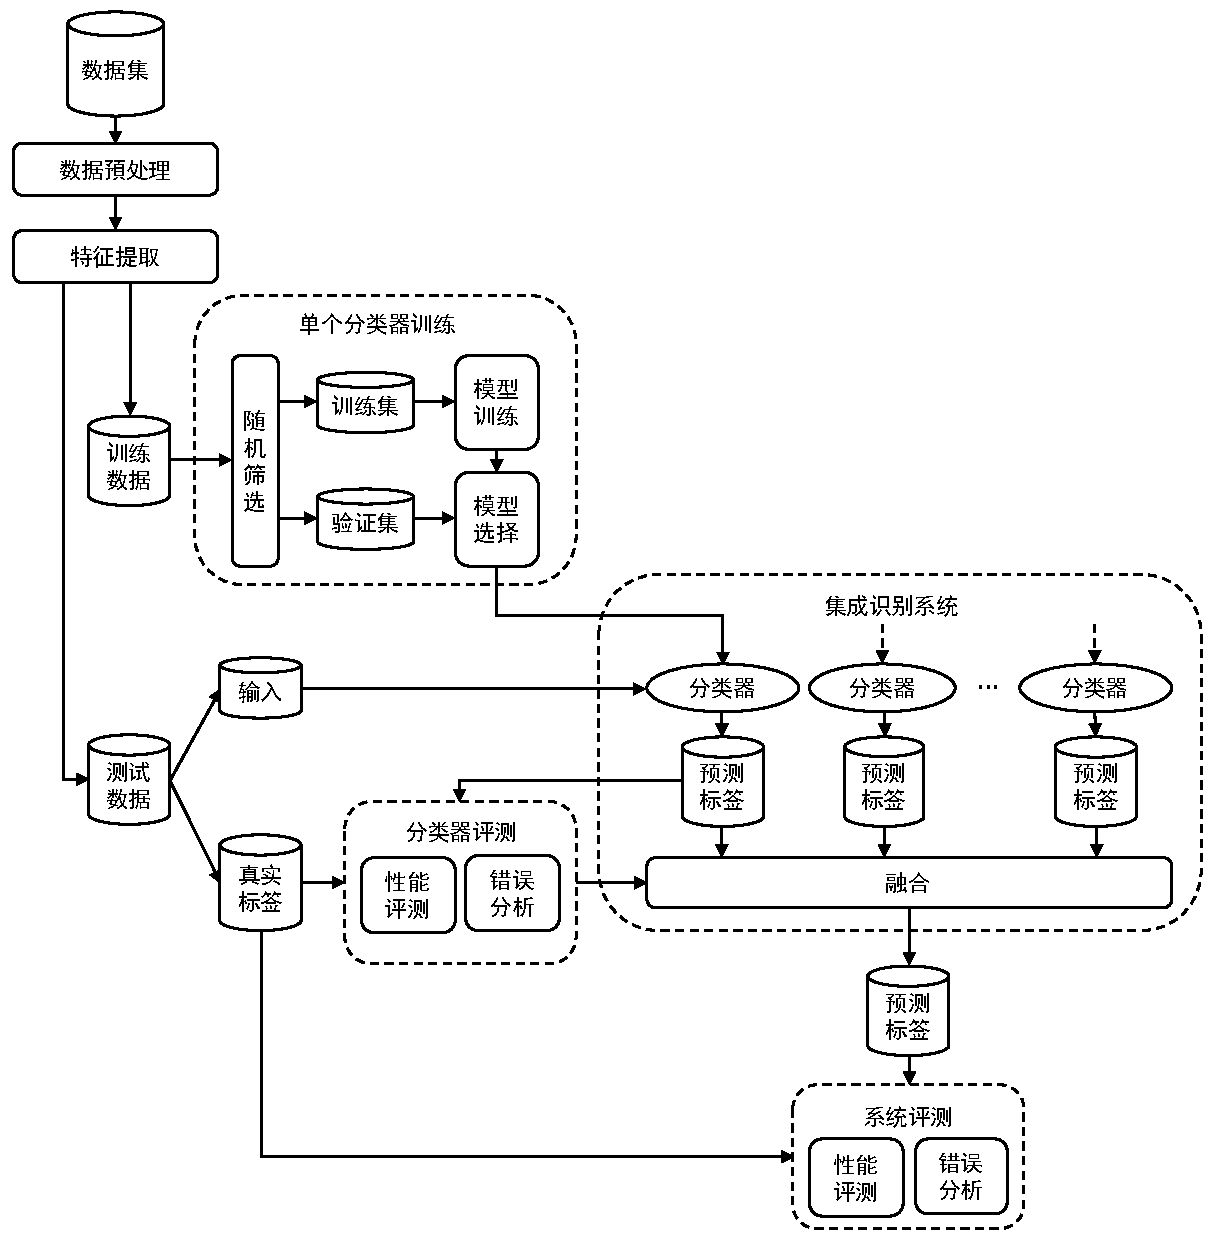
\includegraphics[width=\textwidth]{img/framework.pdf}
  \caption{意图识别的研究框架}
  \label{fig:framework}
\end{figure}

\section{研究框架}
\label{sec:global_framework}

在本小节,我们将根据前述的形式化表示给出一个意图识别的研究框架。由于在本论文的后续研究均面向英语社交媒体文本的分类问题,我们会针对此研究方法对框架进行细化,从原始文本的输入到最终识别目标的输出,理清其中每个步骤的功能和目的,给出一个集成系统的设计框架。针对不同的应用的场景,在后续实验章节中将给出具体的实现方案。

\subsection{框架入口}

图~\ref{fig:framework}显示本文面向意图识别的研究框架。整个框架的输入是实验的数据集,数据集的每个样本包含三个元素,分别是研究的主体、背景信息和意图的倾向。参考前一小节的形式化表示,一个样本可以表示为 $<t, b, c> \in T \times B \times C$。不论是训练数据或测试数据,他们都采用相同的数据预处理技术和特征提取技术来获取样本的特征,以用作分类器的输入,即透过$F_T$和$F_B$分别获取$f_t=F_T(t)$和$f_b=F_B(b)$。

\subsection{基础分类器}

在特征提取完成后,识别模型的输入就准备好了。接下来首先对基础分类器进行研究和分析,比较不同模型和不同参数在对应问题上的整体性能。对于机器学习方法,在模型的训练过程中,需要将训练数据会分成训练集和验证集两个部分。训练集用于调整模型的参数,根据预先设计的损失函数计算模型当前的预测结果和实际标签的偏差,透过微分计算出参数的调整方向,并以一定的学习步长逐步迭代。由于以上训练过程在数学逻辑上是以达到训练集上的最优解来调整参数,会出现对训练样本过拟合的问题,因此会采用验证集来评估模型对训练集以外的样本的识别性能。在每一轮参数调整后计算当前模型在验证集上的性能指标,最后选择其中最优的一轮参数作为该次模型训练最终的参数。

除了分析不同模型在对应问题上的整体性能,透过对被分类器错误识别的样本进行观察,我们需要分析单个分类器的性能局限在哪,分类器对哪些类别的样本有更高的正确率或召回率,哪些样本之间容易出现混淆,或者在输入数据当中是否存在一些有关键信息的特征没有被成功提取。特别地意图识别的研究课题中,我们会关注数据集标签的正确性。在实验的过程中我们假设标签是正确,但有研究指出自动标注会引入噪声\cite{littlestone1988learning},人工标注则难以避免地存在主观性。虽然对不同算法之间的性能比较影响不大,但对于技术水平的评估有其分析的价值。

\subsection{集成识别系统}

经过对基础分类器的分析后,我们对不同模型的识别性能有了深入的了解。为了进一步达到更好的性能,
下一步是基于基础分类器研究集成识别系统的策略和设计。我们提出了一种集成系统的设计方案,结合多个模型相同的分类器的预测结果来作出最终判断,旨在只使用一种模型的基础上尽可能提升识别的性能,或针对特定的性能指标对整个系统的识别倾向进行调整。参考决策树,其识别过程可以认为是一系列的决策,每一步决策都建立在前一步的决策结果上,并且只关注原始问题中的子问题。类似地,我们提出的集成系统经过多次决策来对样本进行意图识别,第一步先由一个分类器或多个分类器的预测结果融合得到一个基础的预测结果,接下来的每一步需要先对前一步的混淆矩阵进行分析,根据哪些类别的样本被误判对指标的影响较大,设定一个子识别任务,从训练数据中筛选出相关的子集来训练新的基础分类器,得出针对该子识别任务的决策结果,决定是否修改上一步中的预测结果。这一方法的原理在于相同的模型在相同配置下的拟合能力是有限的,而子识别任务是原始问题的简化,模型可以专注于拟合一个局部问题,并对前一步的预测结果提出修改意见,起着补丁的作用。具体方法将在后续实验章节中给出详细说明。

同样地,我们需要分析集成系统的性能。在测试数据上,观察系统经过每一轮决策调整之后的识别性能变化,验证系统框架的设计是否满足假设。另外深入观察混淆矩阵的变化,分析各个子识别任务有效的原因,判断其适用和不适用的场景。

\section{本章小结}

在本章我们首先对意图识别给出统一的形式化表示,引出了其中涉及的各个元素并描述他们的相互关系。然后描述了我们面向意图识别的研究框架,其中包括了两个研究重点。一是研究以不同算法得到的分类器对研究问题的整体性能,并作深入的分析,包括单个算法对不同类别样本的识别能力、比较不同算法在不同指标上的区别以理解他们的拟合倾向、观察被错误识别的样本并找出其原因等。二是研究基于基础分类器的集成系统,鉴于单个分类器的识别能力有限,我们提出了一个集成系统的设计方案,旨在结合多个基础分类器的预测结果来得出最终的判断,从而充分发挥一个数学模型的拟合能力,细节实现方法将在后续具体的应用场景中给出说明。




\chapter{意图识别技术}
\label{cha:tech}

\section{本章引论}

根据前一章中描述的研究框架,在本章中我们将针对每一个功能介绍对应的技术实现,其中包括文本预处理、词特征提取、分类算法、集成学习。对后续实验用中使用到的技术给出相对充分的说明,同时也会相关的技术给出概要的描述,以便于其他研究者在本论文未深入探索的方向作出拓展性的研究。

\section{文本预处理}

文本的预处理是所有面向文本的研究的第一步,其目的是为特征提取做好准备。良好的预处理策略可以在尽可能不掉失重要信息的情况下对样本数据进行简化,增加样本之间重复的模式,减轻模型对数据进行拟合的负担,同时更有效地找出数据之间的相互关系。错误的预处理策略会会掉失具有区分能力的信息,甚至产生具有误导性的样本。对于不同的语言,由于其天然的性质不同,预处理的方法也会各异,以下会重点介绍针对社交媒体上英语文本的预处理技术。

\subsection{分词}

为了从文本提取词级别的特征,我们需要首先将句子切成多个词的序列。

虽然对于英语及大部分欧洲语言,空格隔开的字符必然属于不同的词组,但对于不以空格分隔词组的语言(如中文),分词的作用尤其重要。在某些情况下,分词的结果会影响对句子的理解,如将“乒乓球拍卖完了”切割成“乒乓球拍-卖-完-了”或“乒乓球-拍卖-完-了”,对主体应该是“乒乓球拍”还是“乒乓球”,动词应该是“卖”还是“拍卖”,仅凭字面意思无法确定发言者想表达的意思。特别地社交媒体平台上,新词不断的出现,要正确进行分词就有其独特的难点。而分词并不只针对语言中的单词,还针对标点符号或其他特征字符组成的有特殊语义或情感的字符组合,如现今社交媒体上普遍用多个字符拼接成颜文字,其中最常见的微笑的表情“:)”和伤心的表情“:(”,但如果在分词过程中把前者分割成“:”和“)”就会失去其所带的正向情感信息,这在短文本的情感识别中非常关键。

虽然利用空格和标点符号在大部分情况下可以完成对英语句子的分词,但在一些情况下,标点符号作用为词组的一部分而不是词组的分隔符,而在社交媒体上会有空格被省略的情况,以下是一些需要额外处理的情况\cite{jackson2007natural}\cite{mitkov2004oxford}。一是带句号的缩写,如“U.S.”,“.com”,句号应该作为词的一部分,或按句号切割“U.S.”将失去其语义。二是具有一定格式的带标点符号的词组,如电子邮箱地址(如example@email.com)、时间(如 Jan 6th、06/01/19)、电话号码(如(123)456-7890)、网页地址(如www.example.com)等,而在大部分情况下,我们会优先关注这个字符串指的是什么类型的事物而不是细节,譬如将一个句子中的电子邮箱地址或电话号码作替换并不会改变其情感的表达,但识别出一个字符串对应的事情类型,并在清楚它对意图识别没有关联的情况下对其忽略是有意义的。第三种情况是附属词,如“'t”对应“not”,只有正确识别“'”的作用才能识别出否定的意思,否则句子的意思将完全相反。值得注意的是,对社交媒体平台上的文本,除了以上在正规英语中会出现的情况,还有出现其他特殊情况,如“Y!E!S!”和“N!O!”。这需要对数据首先进行人工观察找出特殊的模式,再对语料库进行统计判断其出现频率,若出现频率较高则新增处理规则将对应模式做转换(如将“Y!E!S!”替换成“YES!!!”)或对问题无关的模式忽略(如国外的微博以“RE:”开头表示回复,并不包含任何情感)。

\subsection{拼写修正}

在处理较正式的文件时,我们一般可以默认其文本满足正规的语言语法,词汇基本都是正确的拼写或故意设计的新词(如杂志专栏作家首创针对英国退出欧盟首创单词“Brexit”)。不过在社交媒体上,拼写不符合传统英语的情况则非常普遍,这些情况可以分成三大类。

第一类是非刻意的拼意错误,由于社交媒体上的文本普遍是非正式的,用户不会刻意去保证文本的语言正确性,他们更关注于表达自己的想法、感情或其他意图。拼写修正技术一般基于统计的方法,对于一个不存在的词汇,尝试对其拼写进行有限次编辑,再评估编辑后的词在其上下文中出现的概率,最后选出可能性最高的一个词作替换。拼写修正技术已相当成熟地被应用于搜索引擎和手机键盘等应用中,读者可参考相关研究\cite{ahmed2009revised}\cite{nejja2015context}了解其细节。

第二种情况是网络上常用的代替用词,如以“thx”、“tnx”代替“thanks”,以“k”代替“ok”,以“cant”代替“can't”。虽然这些用法没有被认可为标准用法,但由于方便而在网络上被传播开成功网民们都能理解的用词。对此应对方法有两种,一是人工建立映射表,把代替用词映射到标准的英语词汇,优点在于可以直接引用标准词汇的语义信息,但缺点是需要人工参与,特别是在网络上新用词不断出现的情况下需要持续的更新。另一种是不做处理,利用机器学习方法从大型语料库中自动学习出它的语义,优点在于省去了人工的部分,缺点在于单词的出现很稀疏,对语料库的依赖很强。

第三种情况是语气加强,如“yeeeees”,“AMAZING”,但对于这一类情况处理的重点不只在于转换成标准用词,而是根据具体的应用问题判断是否要保留这个词存在语气加强的这个信息,譬如在情感识别中,语气加强一般提示了此处的情感需要注意。Baziotis等人\cite{baziotis2017semeval2}的做法是在单词前后添加标签示意,如“yeeeees”替换成“yes <enlongated>”,“AMAZING”替换成“amazing <allcaps>”。

\subsection{规范化}

pass

\section{特征提取}

pass

\subsection{词嵌入}

pass

\subsection{词汇特征} % Lexical Feature 

% 多元语法 n-gram
%   统计数据集中多元语法的词频(TF)和逆文本频率(IDF)
%   取TF-IDF最高的N个多元语法
%   对每个条微博得出一个N维向量, 每一维分别对应一个多元语法,其值为该多元语法在该条微博中的数量乘以该多元语法在整个数据集中的IDF
%   每条微博的向量分别进行归一化
% 单词数量
% 字母数量

\subsection{句法特征} % Syntactic features 

% 对文本中单词转换成词性(Part-of-speech, POS)标注
% 和词汇特征中多元语法一样的计算的TF-IDF特征

\subsection{语义特征} % Semantic features

% 词向量平均和
%   对文本进行分词
%   将单词序列转换成词向量序列
%   取词向量序列的平均和作为特征
% 潜在语义
%   利用潜在语义分析(Latent semantic analysis, LSA)从训练集学习单词间的隐藏概念
%   再分别对测试集各个样本提取隐藏概念
% 词类分布
%   利用布朗聚类(Brown Clustering)对训练集的单词进行聚类(N类)
%   每段文本得出一个N维向量,各维对应该文本中包含该类单词的数量

\subsection{基于人工神经网络}

% 人工神经网络对每一个输入进行预测的中间结果可被认为是该输入的隐藏特征
% 利用不同标注的数据集训练的人工神经网络可以用作对应类型的特征提取,如
%  SemEval2014 Task 9: 标注为文本的正负中性情感
%  SemEval2018 Task 1: 标注为文本中是否分别包含了11种情感


\section{分类算法}

pass

\subsection{传统机器学习方法}

% 支持向量机 Support Vector Machine, SVM
% 决策树 Decision Tree
% 随机森林 Random Forest

\subsection{深度学习方法}

% Gated Recurrent Unit, GRU 
% 长短期记忆网络 Long Short-Term Memory, LSTM
% 双向长短期记忆网络 Bidirectional Long Short-Term Memory, BLSTM
% 卷积神经网络 Convolutional Neural Network CNN

\section{集成学习}

pass

% 后融合
%   结合多个子系统的预测结果,根据特定策略得出新的预测结果

%   多数投票 Majority Voting / Hard Voting
%     每个模型分别给出预测标签
%     取最多模型预测的标签作为最终预测结果

%   加权多数投票 Weighted Majority Vote
%     每个模型分别给出预测标签
%     对这些模型的预测标签进行加权投票,取投票最多的标签作为预测结果

%   加权平均概率投票 Soft Voting
%     每个模型分别给出各个标签的预测概率
%     对每个模型的预测概率进行加权不均,取概率最高的标签作为预测结果


\section{本章小结}

pass


%%% 其它部分
\backmatter

%% 本科生要这几个索引,研究生不要。选择性留下。
% 插图索引
\listoffigures
% 表格索引
\listoftables
% 公式索引
\listofequations


%% 参考文献
% 注意:至少需要引用一篇参考文献,否则下面两行可能引起编译错误。
% 如果不需要参考文献,请将下面两行删除或注释掉。
% 数字式引用
\bibliographystyle{thuthesis-numeric}
% 作者-年份式引用
% \bibliographystyle{thuthesis-author-year}
\bibliography{ref/refs}


%% 致谢
% 如果使用声明扫描页,将可选参数指定为扫描后的 PDF 文件名,例如:
% \begin{acknowledgement}[scan-statement.pdf]
\begin{acknowledgement}

衷心感谢导师徐明星副教授多年来对本人的指导和帮助,使我在研究生期间的三年受益匪浅。徐老师在科研问题上有独特的想法,对于我主要研究的自然语言处理领域,当很多研究都专注于采用更复杂的模型进行尝试时,徐老师强调从语言的本质入手,除了亲自翻查语言学的相关材料,还会向心理学的老师谈讨交流,这种对研究的热情和好奇心对我有很大的感染力。除了学术以外,徐老师还会有一些为人处事方面的教导,确实做到了授业与解惑。在此再次表示由衷的感谢。

另外感谢在读期间帮过我的各位老师和同学,因为有你们的帮助使得我读研的三年过得更顺利。感谢家人在背后的支持,让我没有顾虑远离家乡完成我的学业。最后感谢每一位和我非常亲密的好友,在我完全学业期间充满压力的时候,是你们的支持帮我度过了这些困难的时刻。

最后再次向以上的各位表示衷心的感谢。

% 在美国麻省理工学院化学系进行九个月的合作研究期间,承蒙 xxx 教授热心指导与帮助,不胜感激。感谢 xx 实验室主任 xx 教授,以及实验室全体老师和同学们的热情帮助和支持!本课题承蒙国家自然科学基金资助,特此致谢。

% 感谢 \LaTeX 和 \thuthesis\cite{thuthesis},帮我节省了不少时间。
\end{acknowledgement}


%% 附录
\begin{appendix}
\chapter{外文资料原文}
\label{cha:engorg}

\title{The title of the English paper}

\textbf{Abstract:} As one of the most widely used techniques in operations
research, \emph{ mathematical programming} is defined as a means of maximizing a
quantity known as \emph{bjective function}, subject to a set of constraints
represented by equations and inequalities. Some known subtopics of mathematical
programming are linear programming, nonlinear programming, multiobjective
programming, goal programming, dynamic programming, and multilevel
programming$^{[1]}$.

It is impossible to cover in a single chapter every concept of mathematical
programming. This chapter introduces only the basic concepts and techniques of
mathematical programming such that readers gain an understanding of them
throughout the book$^{[2,3]}$.


\section{Single-Objective Programming}
The general form of single-objective programming (SOP) is written
as follows,
\begin{equation}\tag*{(123)} % 如果附录中的公式不想让它出现在公式索引中,那就请
                             % 用 \tag*{xxxx}
\left\{\begin{array}{l}
\max \,\,f(x)\\[0.1 cm]
\mbox{subject to:} \\ [0.1 cm]
\qquad g_j(x)\le 0,\quad j=1,2,\cdots,p
\end{array}\right.
\end{equation}
which maximizes a real-valued function $f$ of
$x=(x_1,x_2,\cdots,x_n)$ subject to a set of constraints.

\newtheorem{mpdef}{Definition}[chapter]
\begin{mpdef}
In SOP, we call $x$ a decision vector, and
$x_1,x_2,\cdots,x_n$ decision variables. The function
$f$ is called the objective function. The set
\begin{equation}\tag*{(456)} % 这里同理,其它不再一一指定。
S=\left\{x\in\Re^n\bigm|g_j(x)\le 0,\,j=1,2,\cdots,p\right\}
\end{equation}
is called the feasible set. An element $x$ in $S$ is called a
feasible solution.
\end{mpdef}

\newtheorem{mpdefop}[mpdef]{Definition}
\begin{mpdefop}
A feasible solution $x^*$ is called the optimal
solution of SOP if and only if
\begin{equation}
f(x^*)\ge f(x)
\end{equation}
for any feasible solution $x$.
\end{mpdefop}

One of the outstanding contributions to mathematical programming was known as
the Kuhn-Tucker conditions\ref{eq:ktc}. In order to introduce them, let us give
some definitions. An inequality constraint $g_j(x)\le 0$ is said to be active at
a point $x^*$ if $g_j(x^*)=0$. A point $x^*$ satisfying $g_j(x^*)\le 0$ is said
to be regular if the gradient vectors $\nabla g_j(x)$ of all active constraints
are linearly independent.

Let $x^*$ be a regular point of the constraints of SOP and assume that all the
functions $f(x)$ and $g_j(x),j=1,2,\cdots,p$ are differentiable. If $x^*$ is a
local optimal solution, then there exist Lagrange multipliers
$\lambda_j,j=1,2,\cdots,p$ such that the following Kuhn-Tucker conditions hold,
\begin{equation}
\label{eq:ktc}
\left\{\begin{array}{l}
    \nabla f(x^*)-\sum\limits_{j=1}^p\lambda_j\nabla g_j(x^*)=0\\[0.3cm]
    \lambda_jg_j(x^*)=0,\quad j=1,2,\cdots,p\\[0.2cm]
    \lambda_j\ge 0,\quad j=1,2,\cdots,p.
\end{array}\right.
\end{equation}
If all the functions $f(x)$ and $g_j(x),j=1,2,\cdots,p$ are convex and
differentiable, and the point $x^*$ satisfies the Kuhn-Tucker conditions
(\ref{eq:ktc}), then it has been proved that the point $x^*$ is a global optimal
solution of SOP.

\subsection{Linear Programming}
\label{sec:lp}

If the functions $f(x),g_j(x),j=1,2,\cdots,p$ are all linear, then SOP is called
a {\em linear programming}.

The feasible set of linear is always convex. A point $x$ is called an extreme
point of convex set $S$ if $x\in S$ and $x$ cannot be expressed as a convex
combination of two points in $S$. It has been shown that the optimal solution to
linear programming corresponds to an extreme point of its feasible set provided
that the feasible set $S$ is bounded. This fact is the basis of the {\em simplex
  algorithm} which was developed by Dantzig as a very efficient method for
solving linear programming.
\begin{table}[ht]
\centering
  \centering
  \caption*{Table~1\hskip1em This is an example for manually numbered table, which
    would not appear in the list of tables}
  \label{tab:badtabular2}
  \begin{tabular}[c]{|m{1.5cm}|c|c|c|c|c|c|}\hline
    \multicolumn{2}{|c|}{Network Topology} & \# of nodes &
    \multicolumn{3}{c|}{\# of clients} & Server \\\hline
    GT-ITM & Waxman Transit-Stub & 600 &
    \multirow{2}{2em}{2\%}&
    \multirow{2}{2em}{10\%}&
    \multirow{2}{2em}{50\%}&
    \multirow{2}{1.2in}{Max. Connectivity}\\\cline{1-3}
    \multicolumn{2}{|c|}{Inet-2.1} & 6000 & & & &\\\hline
    \multirow{2}{1.5cm}{Xue} & Rui  & Ni &\multicolumn{4}{c|}{\multirow{2}*{\thuthesis}}\\\cline{2-3}
    & \multicolumn{2}{c|}{ABCDEF} &\multicolumn{4}{c|}{} \\\hline
\end{tabular}
\end{table}

Roughly speaking, the simplex algorithm examines only the extreme points of the
feasible set, rather than all feasible points. At first, the simplex algorithm
selects an extreme point as the initial point. The successive extreme point is
selected so as to improve the objective function value. The procedure is
repeated until no improvement in objective function value can be made. The last
extreme point is the optimal solution.

\subsection{Nonlinear Programming}

If at least one of the functions $f(x),g_j(x),j=1,2,\cdots,p$ is nonlinear, then
SOP is called a {\em nonlinear programming}.

A large number of classical optimization methods have been developed to treat
special-structural nonlinear programming based on the mathematical theory
concerned with analyzing the structure of problems.
\begin{figure}[h]
  \centering
  
\includegraphics{thu-lib-logo}
  \caption*{Figure~1\quad This is an example for manually numbered figure,
    which would not appear in the list of figures}
  \label{tab:badfigure2}
\end{figure}

Now we consider a nonlinear programming which is confronted solely with
maximizing a real-valued function with domain $\Re^n$.  Whether derivatives are
available or not, the usual strategy is first to select a point in $\Re^n$ which
is thought to be the most likely place where the maximum exists. If there is no
information available on which to base such a selection, a point is chosen at
random. From this first point an attempt is made to construct a sequence of
points, each of which yields an improved objective function value over its
predecessor. The next point to be added to the sequence is chosen by analyzing
the behavior of the function at the previous points. This construction continues
until some termination criterion is met. Methods based upon this strategy are
called {\em ascent methods}, which can be classified as {\em direct methods},
{\em gradient methods}, and {\em Hessian methods} according to the information
about the behavior of objective function $f$. Direct methods require only that
the function can be evaluated at each point. Gradient methods require the
evaluation of first derivatives of $f$. Hessian methods require the evaluation
of second derivatives. In fact, there is no superior method for all
problems. The efficiency of a method is very much dependent upon the objective
function.

\subsection{Integer Programming}

{\em Integer programming} is a special mathematical programming in which all of
the variables are assumed to be only integer values. When there are not only
integer variables but also conventional continuous variables, we call it {\em
  mixed integer programming}. If all the variables are assumed either 0 or 1,
then the problem is termed a {\em zero-one programming}. Although integer
programming can be solved by an {\em exhaustive enumeration} theoretically, it
is impractical to solve realistically sized integer programming problems. The
most successful algorithm so far found to solve integer programming is called
the {\em branch-and-bound enumeration} developed by Balas (1965) and Dakin
(1965). The other technique to integer programming is the {\em cutting plane
  method} developed by Gomory (1959).

\hfill\textit{Uncertain Programming\/}\quad(\textsl{BaoDing Liu, 2006.2})

\section*{References}
\noindent{\itshape NOTE: These references are only for demonstration. They are
  not real citations in the original text.}

\begin{translationbib}
\item Donald E. Knuth. The \TeX book. Addison-Wesley, 1984. ISBN: 0-201-13448-9
\item Paul W. Abrahams, Karl Berry and Kathryn A. Hargreaves. \TeX\ for the
  Impatient. Addison-Wesley, 1990. ISBN: 0-201-51375-7
\item David Salomon. The advanced \TeX book.  New York : Springer, 1995. ISBN:0-387-94556-3
\end{translationbib}

\chapter{外文资料的调研阅读报告或书面翻译}

\title{英文资料的中文标题}

{\heiti 摘要:} 本章为外文资料翻译内容。如果有摘要可以直接写上来,这部分好像没有
明确的规定。

\section{单目标规划}
北冥有鱼,其名为鲲。鲲之大,不知其几千里也。化而为鸟,其名为鹏。鹏之背,不知其几
千里也。怒而飞,其翼若垂天之云。是鸟也,海运则将徙于南冥。南冥者,天池也。
\begin{equation}\tag*{(123)}
 p(y|\mathbf{x}) = \frac{p(\mathbf{x},y)}{p(\mathbf{x})}=
\frac{p(\mathbf{x}|y)p(y)}{p(\mathbf{x})}
\end{equation}

吾生也有涯,而知也无涯。以有涯随无涯,殆已!已而为知者,殆而已矣!为善无近名,为
恶无近刑,缘督以为经,可以保身,可以全生,可以养亲,可以尽年。

\subsection{线性规划}
庖丁为文惠君解牛,手之所触,肩之所倚,足之所履,膝之所倚,砉然响然,奏刀騞然,莫
不中音,合于桑林之舞,乃中经首之会。
\begin{table}[ht]
\centering
  \centering
  \caption*{表~1\hskip1em 这是手动编号但不出现在索引中的一个表格例子}
  \label{tab:badtabular3}
  \begin{tabular}[c]{|m{1.5cm}|c|c|c|c|c|c|}\hline
    \multicolumn{2}{|c|}{Network Topology} & \# of nodes &
    \multicolumn{3}{c|}{\# of clients} & Server \\\hline
    GT-ITM & Waxman Transit-Stub & 600 &
    \multirow{2}{2em}{2\%}&
    \multirow{2}{2em}{10\%}&
    \multirow{2}{2em}{50\%}&
    \multirow{2}{1.2in}{Max. Connectivity}\\\cline{1-3}
    \multicolumn{2}{|c|}{Inet-2.1} & 6000 & & & &\\\hline
    \multirow{2}{1.5cm}{Xue} & Rui  & Ni &\multicolumn{4}{c|}{\multirow{2}*{\thuthesis}}\\\cline{2-3}
    & \multicolumn{2}{c|}{ABCDEF} &\multicolumn{4}{c|}{} \\\hline
\end{tabular}
\end{table}

文惠君曰:“嘻,善哉!技盖至此乎?”庖丁释刀对曰:“臣之所好者道也,进乎技矣。始臣之
解牛之时,所见无非全牛者;三年之后,未尝见全牛也;方今之时,臣以神遇而不以目视,
官知止而神欲行。依乎天理,批大郤,导大窾,因其固然。技经肯綮之未尝,而况大坬乎!
良庖岁更刀,割也;族庖月更刀,折也;今臣之刀十九年矣,所解数千牛矣,而刀刃若新发
于硎。彼节者有间而刀刃者无厚,以无厚入有间,恢恢乎其于游刃必有余地矣。是以十九年
而刀刃若新发于硎。虽然,每至于族,吾见其难为,怵然为戒,视为止,行为迟,动刀甚微,
謋然已解,如土委地。提刀而立,为之而四顾,为之踌躇满志,善刀而藏之。”

文惠君曰:“善哉!吾闻庖丁之言,得养生焉。”


\subsection{非线性规划}
孔子与柳下季为友,柳下季之弟名曰盗跖。盗跖从卒九千人,横行天下,侵暴诸侯。穴室枢
户,驱人牛马,取人妇女。贪得忘亲,不顾父母兄弟,不祭先祖。所过之邑,大国守城,小
国入保,万民苦之。孔子谓柳下季曰:“夫为人父者,必能诏其子;为人兄者,必能教其弟。
若父不能诏其子,兄不能教其弟,则无贵父子兄弟之亲矣。今先生,世之才士也,弟为盗
跖,为天下害,而弗能教也,丘窃为先生羞之。丘请为先生往说之。”
\begin{figure}[h]
  \centering
  
\includegraphics{thu-whole-logo}
  \caption*{图~1\hskip1em 这是手动编号但不出现索引中的图片的例子}
  \label{tab:badfigure3}
\end{figure}

柳下季曰:“先生言为人父者必能诏其子,为人兄者必能教其弟,若子不听父之诏,弟不受
兄之教,虽今先生之辩,将奈之何哉?且跖之为人也,心如涌泉,意如飘风,强足以距敌,
辩足以饰非。顺其心则喜,逆其心则怒,易辱人以言。先生必无往。”

孔子不听,颜回为驭,子贡为右,往见盗跖。

\subsection{整数规划}
盗跖乃方休卒徒大山之阳,脍人肝而餔之。孔子下车而前,见谒者曰:“鲁人孔丘,闻将军
高义,敬再拜谒者。”谒者入通。盗跖闻之大怒,目如明星,发上指冠,曰:“此夫鲁国之
巧伪人孔丘非邪?为我告之:尔作言造语,妄称文、武,冠枝木之冠,带死牛之胁,多辞缪
说,不耕而食,不织而衣,摇唇鼓舌,擅生是非,以迷天下之主,使天下学士不反其本,妄
作孝弟,而侥幸于封侯富贵者也。子之罪大极重,疾走归!不然,我将以子肝益昼餔之膳。”


\chapter{其它附录}
前面两个附录主要是给本科生做例子。其它附录的内容可以放到这里,当然如果你愿意,可
以把这部分也放到独立的文件中,然后将其 \cs{input} 到主文件中。

\end{appendix}

%% 个人简历
\begin{resume}

  \resumeitem{个人简历}

  1994 年 6 月 4 日出生于 澳门特别行政区。

  2012 年 9 月考入清华大学计算机科学与技术系,2016 年 7 月本科毕业并获得工学学士学位。

  2016 年 9 月免试进入清华大学计算机科学与技术系攻读硕士学位至今。

  \researchitem{发表的学术论文} % 发表的和录用的合在一起

  % 1. 已经刊载的学术论文(本人是第一作者,或者导师为第一作者本人是第二作者)
  % \begin{publications}
    % \item Yang Y, Ren T L, Zhang L T, et al. Miniature microphone with silicon-based ferroelectric thin films. Integrated Ferroelectrics, 2003, 52:229-235. (SCI 收录, 检索号:758FZ.)
    % \item 杨轶, 张宁欣, 任天令, 等. 硅基铁电微声学器件中薄膜残余应力的研究. 中国机械工程, 2005, 16(14):1289-1291. (EI 收录, 检索号:0534931 2907.)
    % \item 杨轶, 张宁欣, 任天令, 等. 集成铁电器件中的关键工艺研究. 仪器仪表学报, 2003, 24(S4):192-193. (EI 源刊.)
  % \end{publications}

  % 2. 尚未刊载,但已经接到正式录用函的学术论文(本人为第一作者,或者
  %    导师为第一作者本人是第二作者)。
  \begin{publications}[before=\publicationskip,after=\publicationskip]
    % \item Yang Y, Ren T L, Zhu Y P, et al. PMUTs for handwriting recognition. In press. (已被 Integrated Ferroelectrics 录用. SCI 源刊.)

    \item Xihao Liang, Ye Ma, Mingxing Xu. THU-HCSI at SemEval-2019 Task 3: Hierarchical Ensemble Classification of Contextual Emotion in Conversation [C]//Proceedings of The 13th International Workshop on Semantic Evaluation (SemEval-2019). [S.l.: s.n.], 2019: 345-349.

    \item Ye Ma, Xihao Liang, Mingxing Xu. THUHCSI in MediaEval 2018 Emotional Impact of Movies Task[C]//Working Notes Proceedings of the MediaEval 2018 Workshop, Sophia Antipolis, France, 29-31 October 2018. [S.l.: s.n.], 2018.

  \end{publications}

  % 3. 其他学术论文。可列出除上述两种情况以外的其他学术论文,但必须是
  %    已经刊载或者收到正式录用函的论文。
  % \begin{publications}
    % \item Wu X M, Yang Y, Cai J, et al. Measurements of ferroelectric MEMS microphones. Integrated Ferroelectrics, 2005, 69:417-429. (SCI 收录, 检索号:896KM)
    % \item 贾泽, 杨轶, 陈兢, 等. 用于压电和电容微麦克风的体硅腐蚀相关研究. 压电与声光, 2006, 28(1):117-119. (EI 收录, 检索号:06129773469)
    % \item 伍晓明, 杨轶, 张宁欣, 等. 基于MEMS技术的集成铁电硅微麦克风. 中国集成电路, 2003, 53:59-61.
  % \end{publications}

  % \researchitem{研究成果} % 有就写,没有就删除
  % \begin{achievements}
  %   \item 任天令, 杨轶, 朱一平, 等. 硅基铁电微声学传感器畴极化区域控制和电极连接的
  %    方法: 中国, CN1602118A. (中国专利公开号)
  %  \item Ren T L, Yang Y, Zhu Y P, et al. Piezoelectric micro acoustic sensor
  %    based on ferroelectric materials: USA, No.11/215, 102. (美国发明专利申请号)
  %\end{achievements}

  \researchitem{支持本课题研究的科研项目} % 发表的和录用的合在一起

  \begin{achievements}

  \item 国家自然科学基金重点项目:互联网话语理解的心理机制与计算建模(资助号:61433018)

  \item 北京汉迪移动互联网科技股份有限公司合作项目:基于大数据的多媒体信息个性化推荐系统

  \end{achievements}


\end{resume}


%% 本科生进行格式审查是需要下面这个表格,答辩可能不需要。选择性留下。
% 综合论文训练记录表
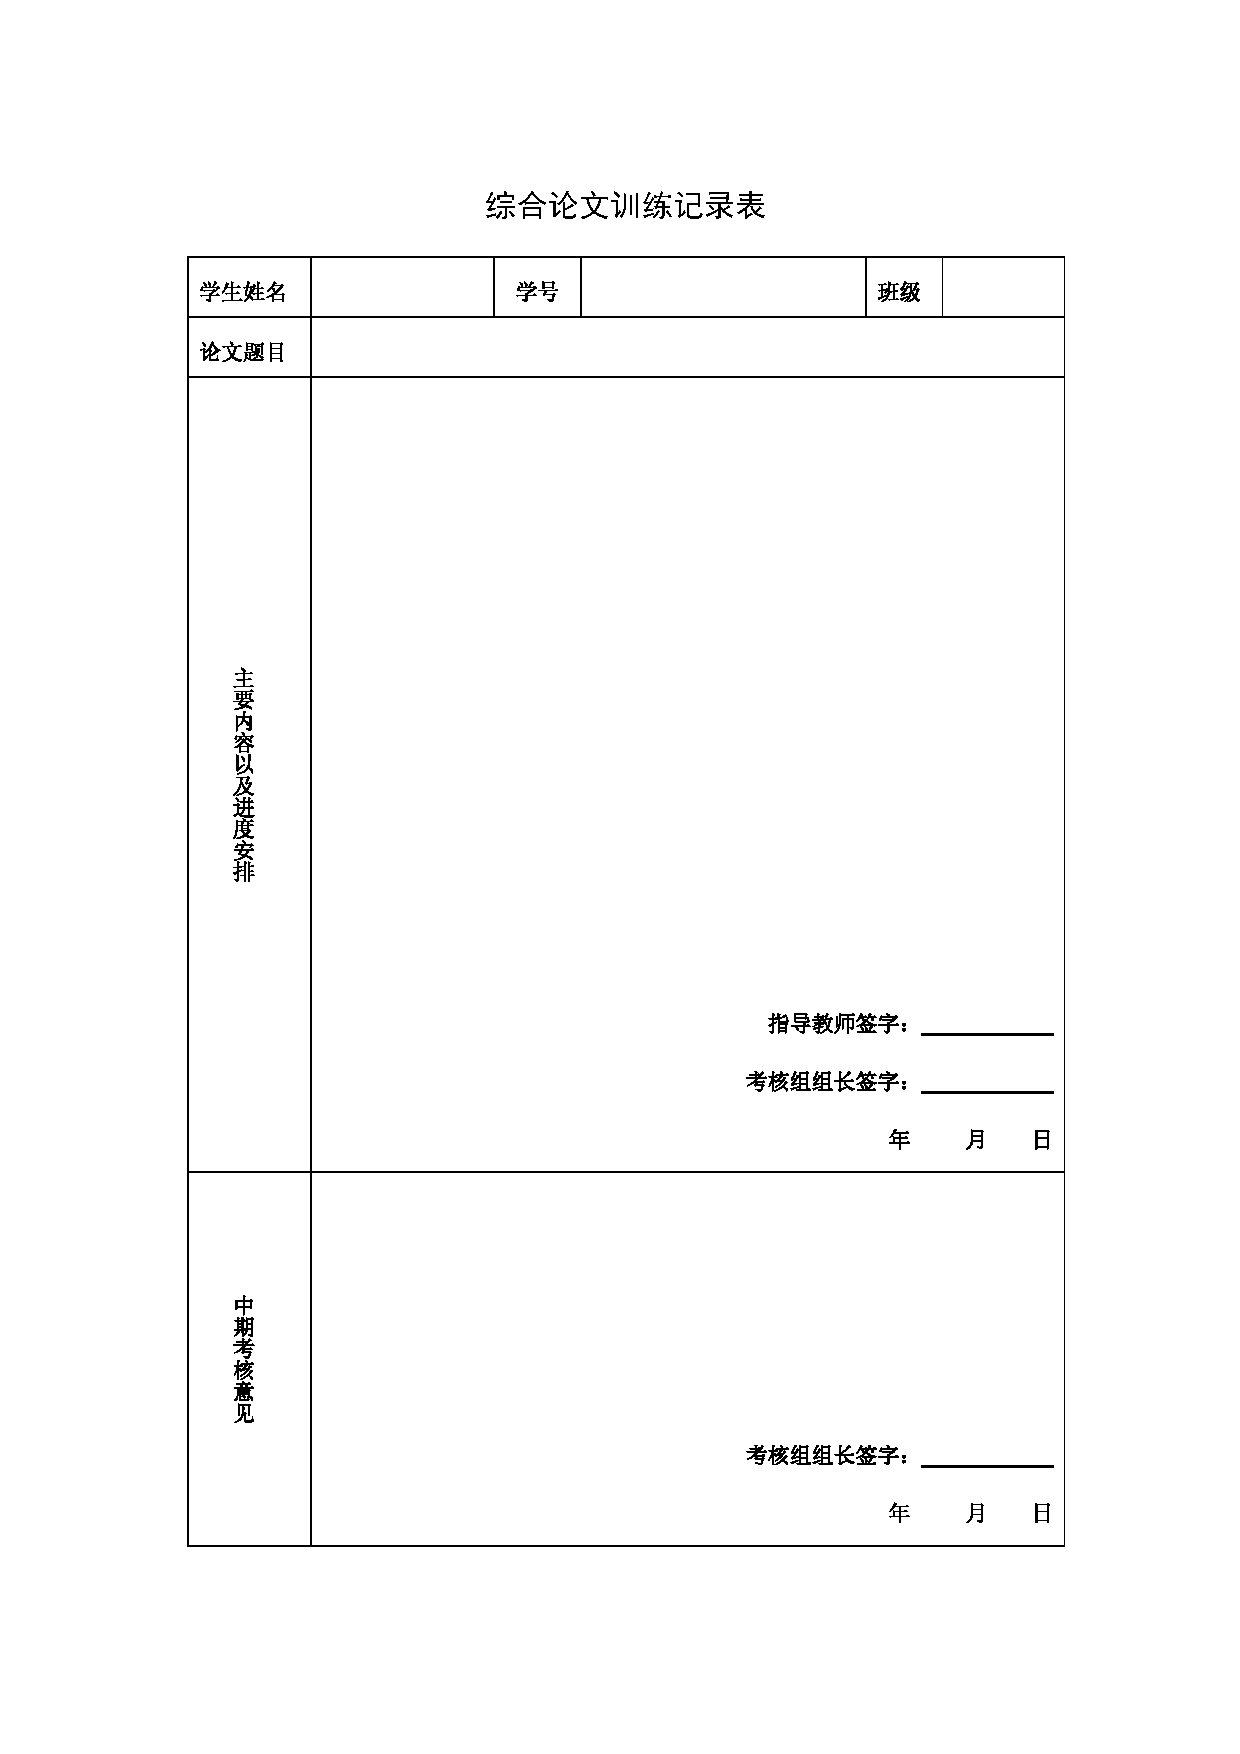
\includepdf[pages=-]{scan-record.pdf}
\end{document}
